\hypertarget{des-alpes-japonaises-de-nagano-uxe0-la-bruxfblante-osaka}{%
\section{Des alpes japonaises de Nagano à la brûlante
Osaka}\label{des-alpes-japonaises-de-nagano-uxe0-la-bruxfblante-osaka}}

\emph{Lundi 16 juillet 2018}

Pour la suite de nos aventures, on a décidé de poser les valises
quelques jours à Nagano, plus en altitude, dans les "Alpes japonaises".
Effectivement, les chalets en bois et la fraîcheur (relative) de l'air
donnent à l'endroit des allures montagnardes, mais les reliefs sont
beaucoup plus...modérés. On s'installe à l'auberge de jeunesse
Moritomizu Backpackers, à deux pas de la gare, pour faciliter les
excursions. Nous y sommes accueillis à la japonaise : \emph{Alors voici
un plan de l'auberge, ici le premier étage, au-dessus le deuxième étage,
puis le troisième. Voici une maquette de votre futon, avec une petite
poupée qui vous représente, qui vous montre qu'il faut bien dormir entre
les deux draps.} Bien. Les doutes sur l'utilisation des draps ayant été
levés, on entame notre première excursion : Kanazawa.

\begin{figure}
\centering
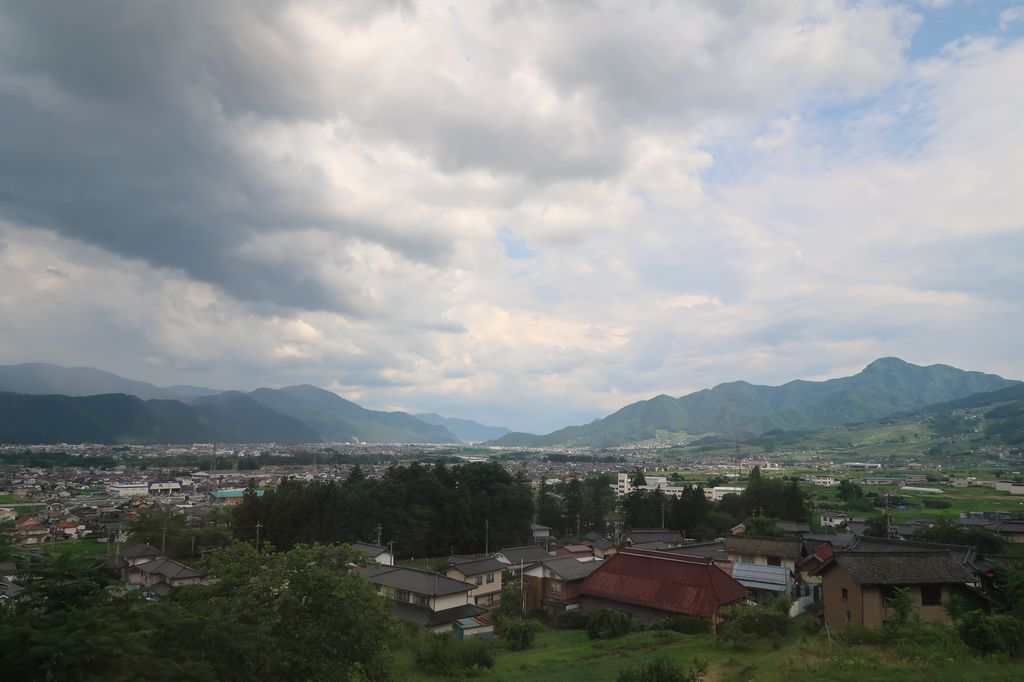
\includegraphics{images/20180723_nagano.JPG}
\caption{Les petites Alpes japonaises, depuis le train.}
\end{figure}

A Kanazawa, on est accueillis par la porte Torii moderne de la gare, le
marché aux poissons en face, et par le prix des fruits, qui nous
surprend toujours ! Ils sont emballés un à un puis placés dans des
boîtes prêtes à poster (voir la photo dans la galerie). On se balade
ensuite dans l'ancien quartier des samouraïs où on visite la maison de
l'un d'eux, havre de tranquilité avec un jardin japonais d'où on a du
mal à partir. Après les samouraïs, les ninjas : le temple de Myoryuji a
été surnommé Ninja-dera, avec ses nombreuses cachettes, trappes
invisibles, escaliers camouflés et autres passages secrets supposés.
Sans oublier la chambre à thé, parce qu'en cas de siège il ne faut pas
oublier ses priorités ! On y a rencontré aussi Frankel, un touriste
d'Atlanta qui fera un bout de chemin avec nous. Après un court passage
au château de Kanazawa, la chaleur nous pousse plutôt vers le parc
Kenroku-en, où on regrette de ne pas être quelques mois plus tôt, à la
saison des cerisiers en fleurs... La journée se finit dans l'élégant
quartier des geishas, que nous n'aurons malheureusement pas le plaisir
de croiser sur notre chemin.

\begin{figure}
\centering
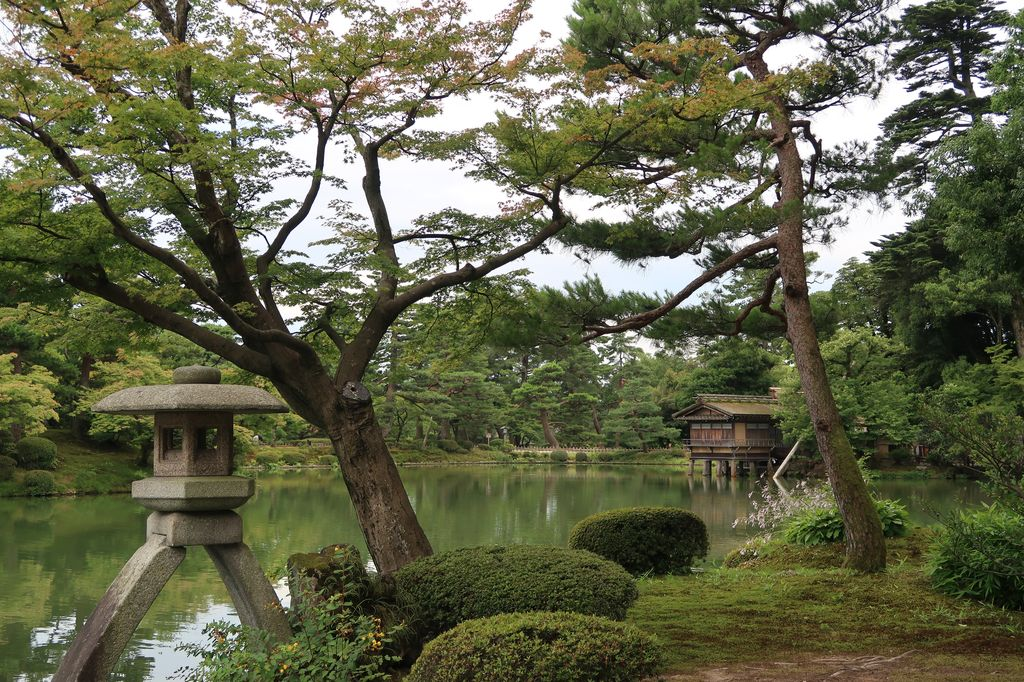
\includegraphics{images/20180723_kanazawa.JPG}
\caption{Le parc Kenroku-en.}
\end{figure}

Le lendemain, on part un peu plus en altitude, à Yamanouchi, où après
une agréable balade en forêt on arrive dans le domaine des macaques des
neiges. En hiver, ils y trouvent une source d'eau chaude pour se
baigner, mais en plein été ils sont surtout attirés par le repas apporté
par les employés du parc. N'empêche qu'ils sont nombreux et toujours
aussi fascinants à observer !

\begin{figure}
\centering
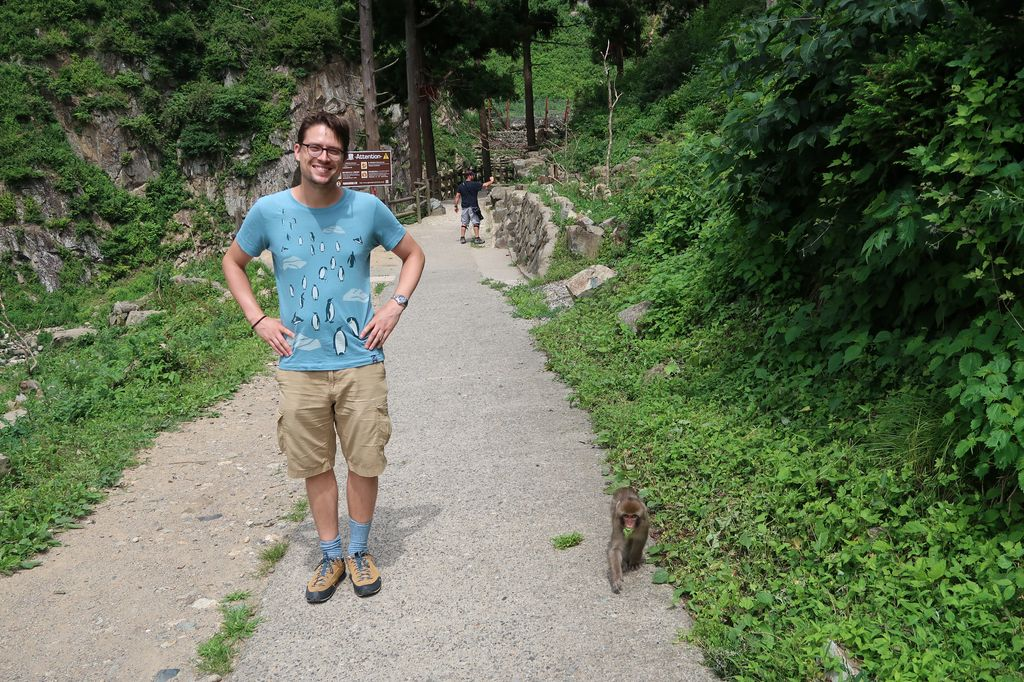
\includegraphics{images/20180723_singes.JPG}
\caption{Balade au milieu des macaques des neiges.}
\end{figure}

Sur le chemin du retour, on s'arrête à Obuse, la ville où le fameux
peintre Hokusai a passé une partie de ses vieilles années, et on
redécouvre ses oeuvres dans le petit musée qui lui est dédié. D'ailleurs
Hokusai a laissé une belle phrase concernant son art du dessin :

\begin{quote}
Depuis l'âge de 6 ans, j'avais la manie de dessiner la forme des objets.
Vers l'âge de 50 ans, j'avais publié une infinité de dessins, mais tout
ce que j'ai produit avant l'âge de 70 ans ne vaut pas la peine d'être
compté. C'est à l'âge de 73 ans que j'ai compris à peu près la structure
de la nature vraie des animaux, des herbes, des arbres, des oiseaux, des
poissons et des insectes. Par conséquent, à l'âge de 80 ans, j'aurai
fait encore plus de progrès ; à 90 ans, je pénétrerai le mystère des
choses ; à 100 ans, je serai certainement parvenu à un stade merveilleux
et, quand j'aurai 110 ans, tout ce que je ferai, un point, une ligne,
sera vivant.
\end{quote}

De retour à Nagano on arrive à la fin du jour au temple Zenko-ji, lieu
de pélerinage bouddhiste. La fin de journée donne un charme particulier
au lieu, où on se balade quasiment seuls. Une averse de pluie nous prend
au dépourvu mais ne fait qu'ajouter à l'ambiance un peu mystérieuse qui
règne.

\begin{figure}
\centering
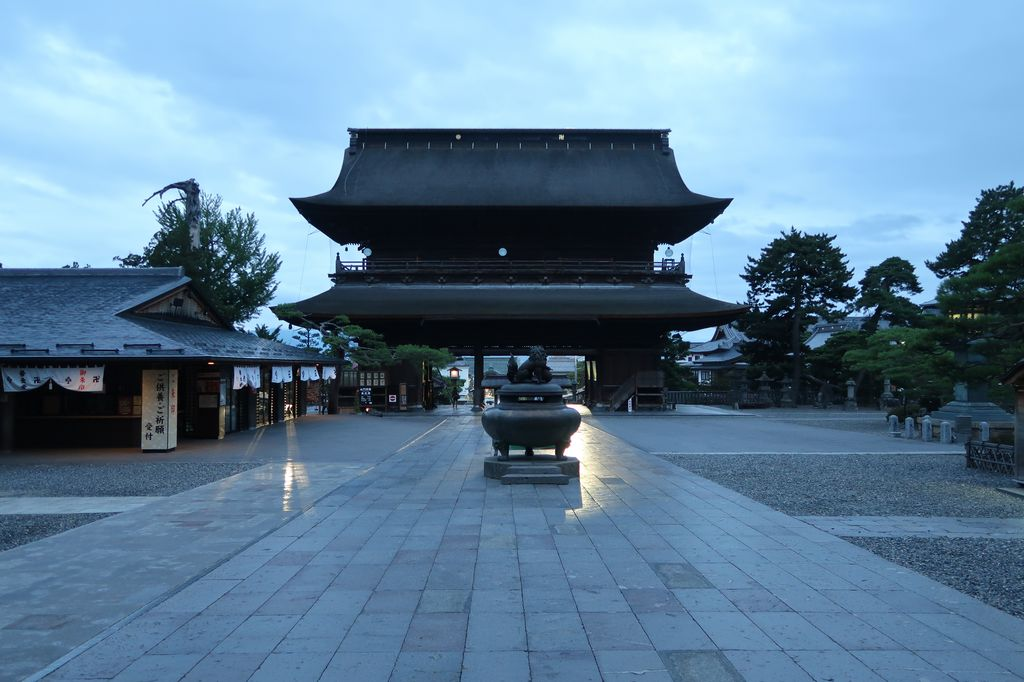
\includegraphics{images/20180723_zenko.JPG}
\caption{Seuls au temple Zenko-ji.}
\end{figure}

En quittant Nagano, un peu à regret, on fait une escale à Matsumoto pour
y visiter son célèbre château noir, l'un des 12 châteaux originaux du
Japon. Le château a donc été rénové mais pas reconstruit de zéro, comme
c'est le cas de très nombreux châteaux détruits principalement pendant
la guerre du Pacifique. On profite de la disponibilité d'un adorable
guide volontaire qui nous raconte l'histoire et les secrets du château,
dans un récit ponctué de blagues et de jeux de mots... inattendus ! Ce
monsieur, d'un certain âge, a d'ailleurs systématiquement salué les
touristes étrangers sur notre passage en leur souhaitant la bienvenue
dans leurs langues respectives (allemand, espagnol, français, danois,
finnois, ...). Il nous a expliqué pouvoir échanger quelques mots dans
plus de vingt langues !

\begin{figure}
\centering
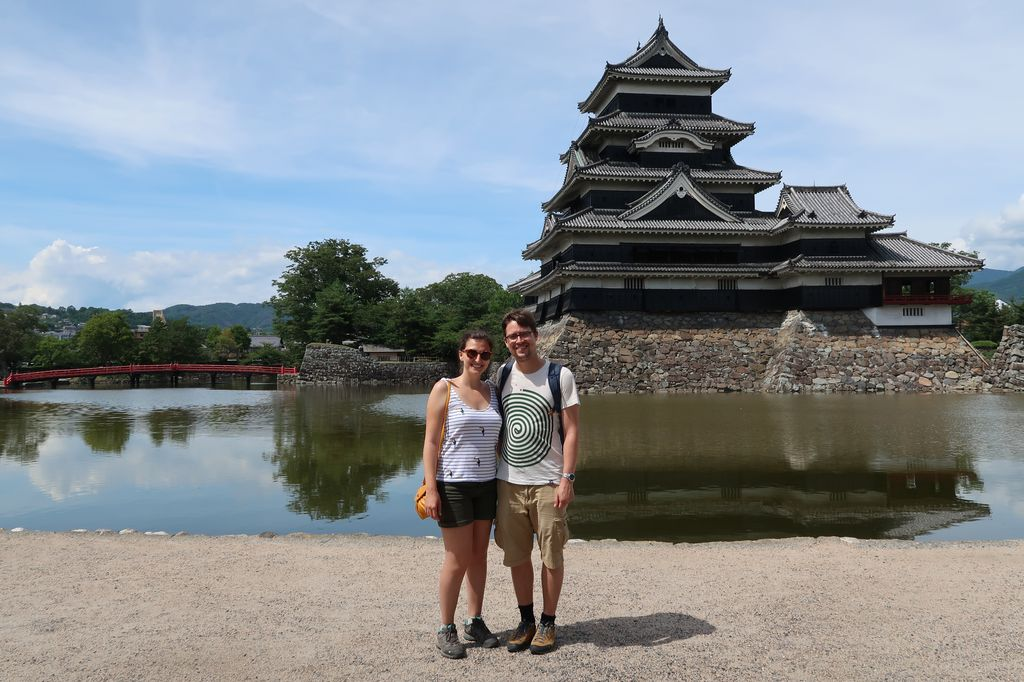
\includegraphics{images/20180723_matsumoto.JPG}
\caption{Devant le château du corbeau, surnom du château de Matsumoto.}
\end{figure}

De retour à Osaka, la chaleur ayant atteint son paroxysme, nous avons
pour la première journée opté pour un programme à l'opposé de tout ce
que nous avions fait jusque là : après une bonne heure de marche (pour
garder le rythme), on a enchaîné shopping/burgers/cinéma : presque
dépaysant ! Mais on ne pouvait pas partir sur une note si peu japonaise
: l'élégant château d'Himeji et ses marches dans tous les sens nous a
mis à l'épreuve avant la longue soirée qui nous attendait. On retiendra
que regarder la victoire de la France en finale de la coupe du monde
dans un pub irlandais à minuit à Osaka, entourés de gens de toutes
nationalités, est une expérience étonnamment riche en émotions.

\begin{figure}
\centering
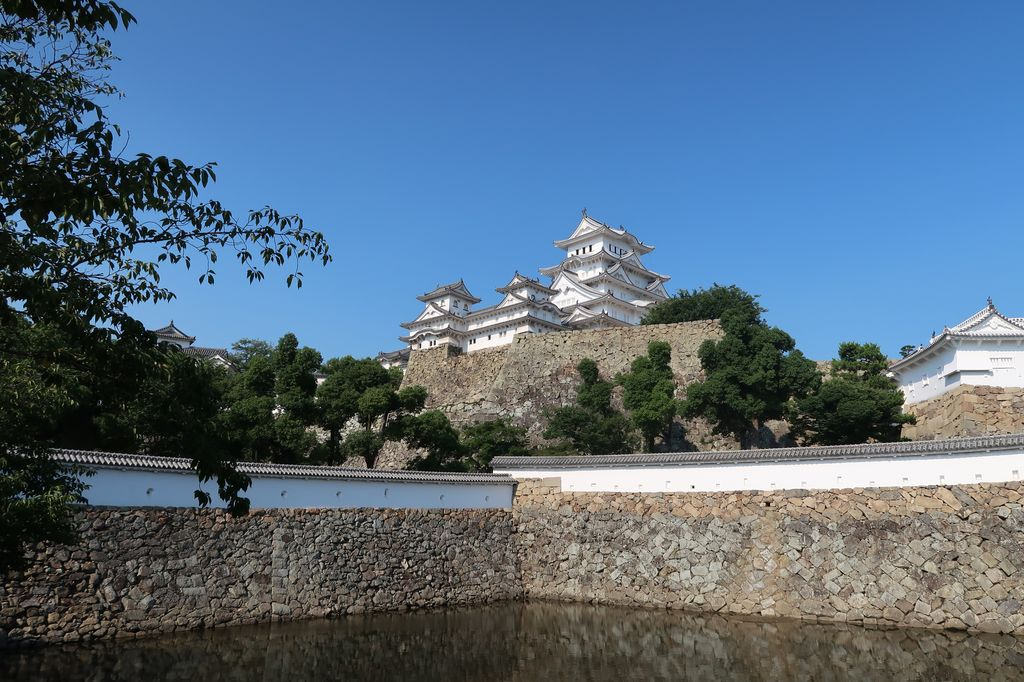
\includegraphics{images/20180723_himeji.JPG}
\caption{L'élégant château d'Himeji, le château du héron blanc.}
\end{figure}

Enfin, avant de quitter Osaka et le Japon, une dernière expérience nous
a attirés : la visite du musée des nouilles instantanées. L'agréable
surprise a été la découverte de l'atelier, où après avoir décoré chacun
sa "cup" de nouilles, on la fait remplir de manière personnalisée, puis
sceller. On n'a pas encore goûté les nôtres, mais on vous en donnera des
nouvelles !

\begin{figure}
\centering
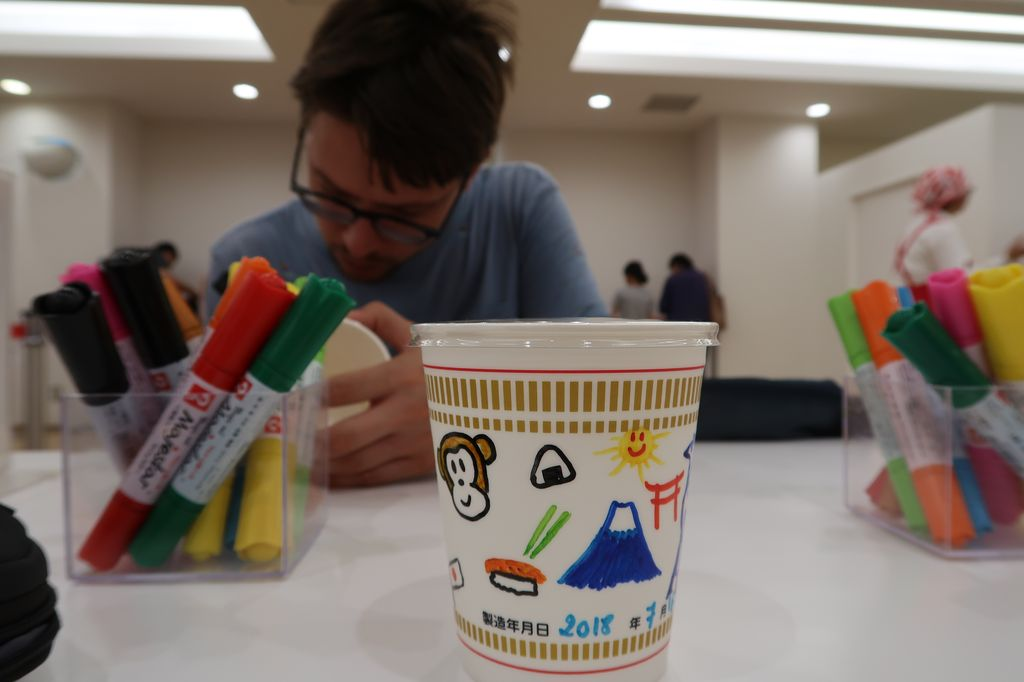
\includegraphics{images/20180723_noodles.JPG}
\caption{Atelier décoration de cup noodles, moment de retour en enfance
!}
\end{figure}

Après un dernier repas de sushis, il est temps de dire au-revoir au
Japon, que je suis heureuse d'avoir enfin découvert (après tout ce que
Flo me racontait tout le temps sur ce pays) et dont je garderai de très
bons souvenirs. Et de dire au-revoir à Marianne, que nous retrouverons à
la fin de notre séjour, au Canada, et qui nous a débarrassés d'un sac
d'affaires qui nous ont peu ou pas servies. On voyage encore plus léger
désormais !

Merci mille fois à tous nos hôtes franco-japonais, avec qui nous avons
passé de très agréables moments. A bientôt pour les prochaines
aventures, dans l'hémisphère Sud cette fois...

\textbf{bonus} Et voici la carte récapitulative de nos destinations au
Japon :

\begin{figure}
\centering
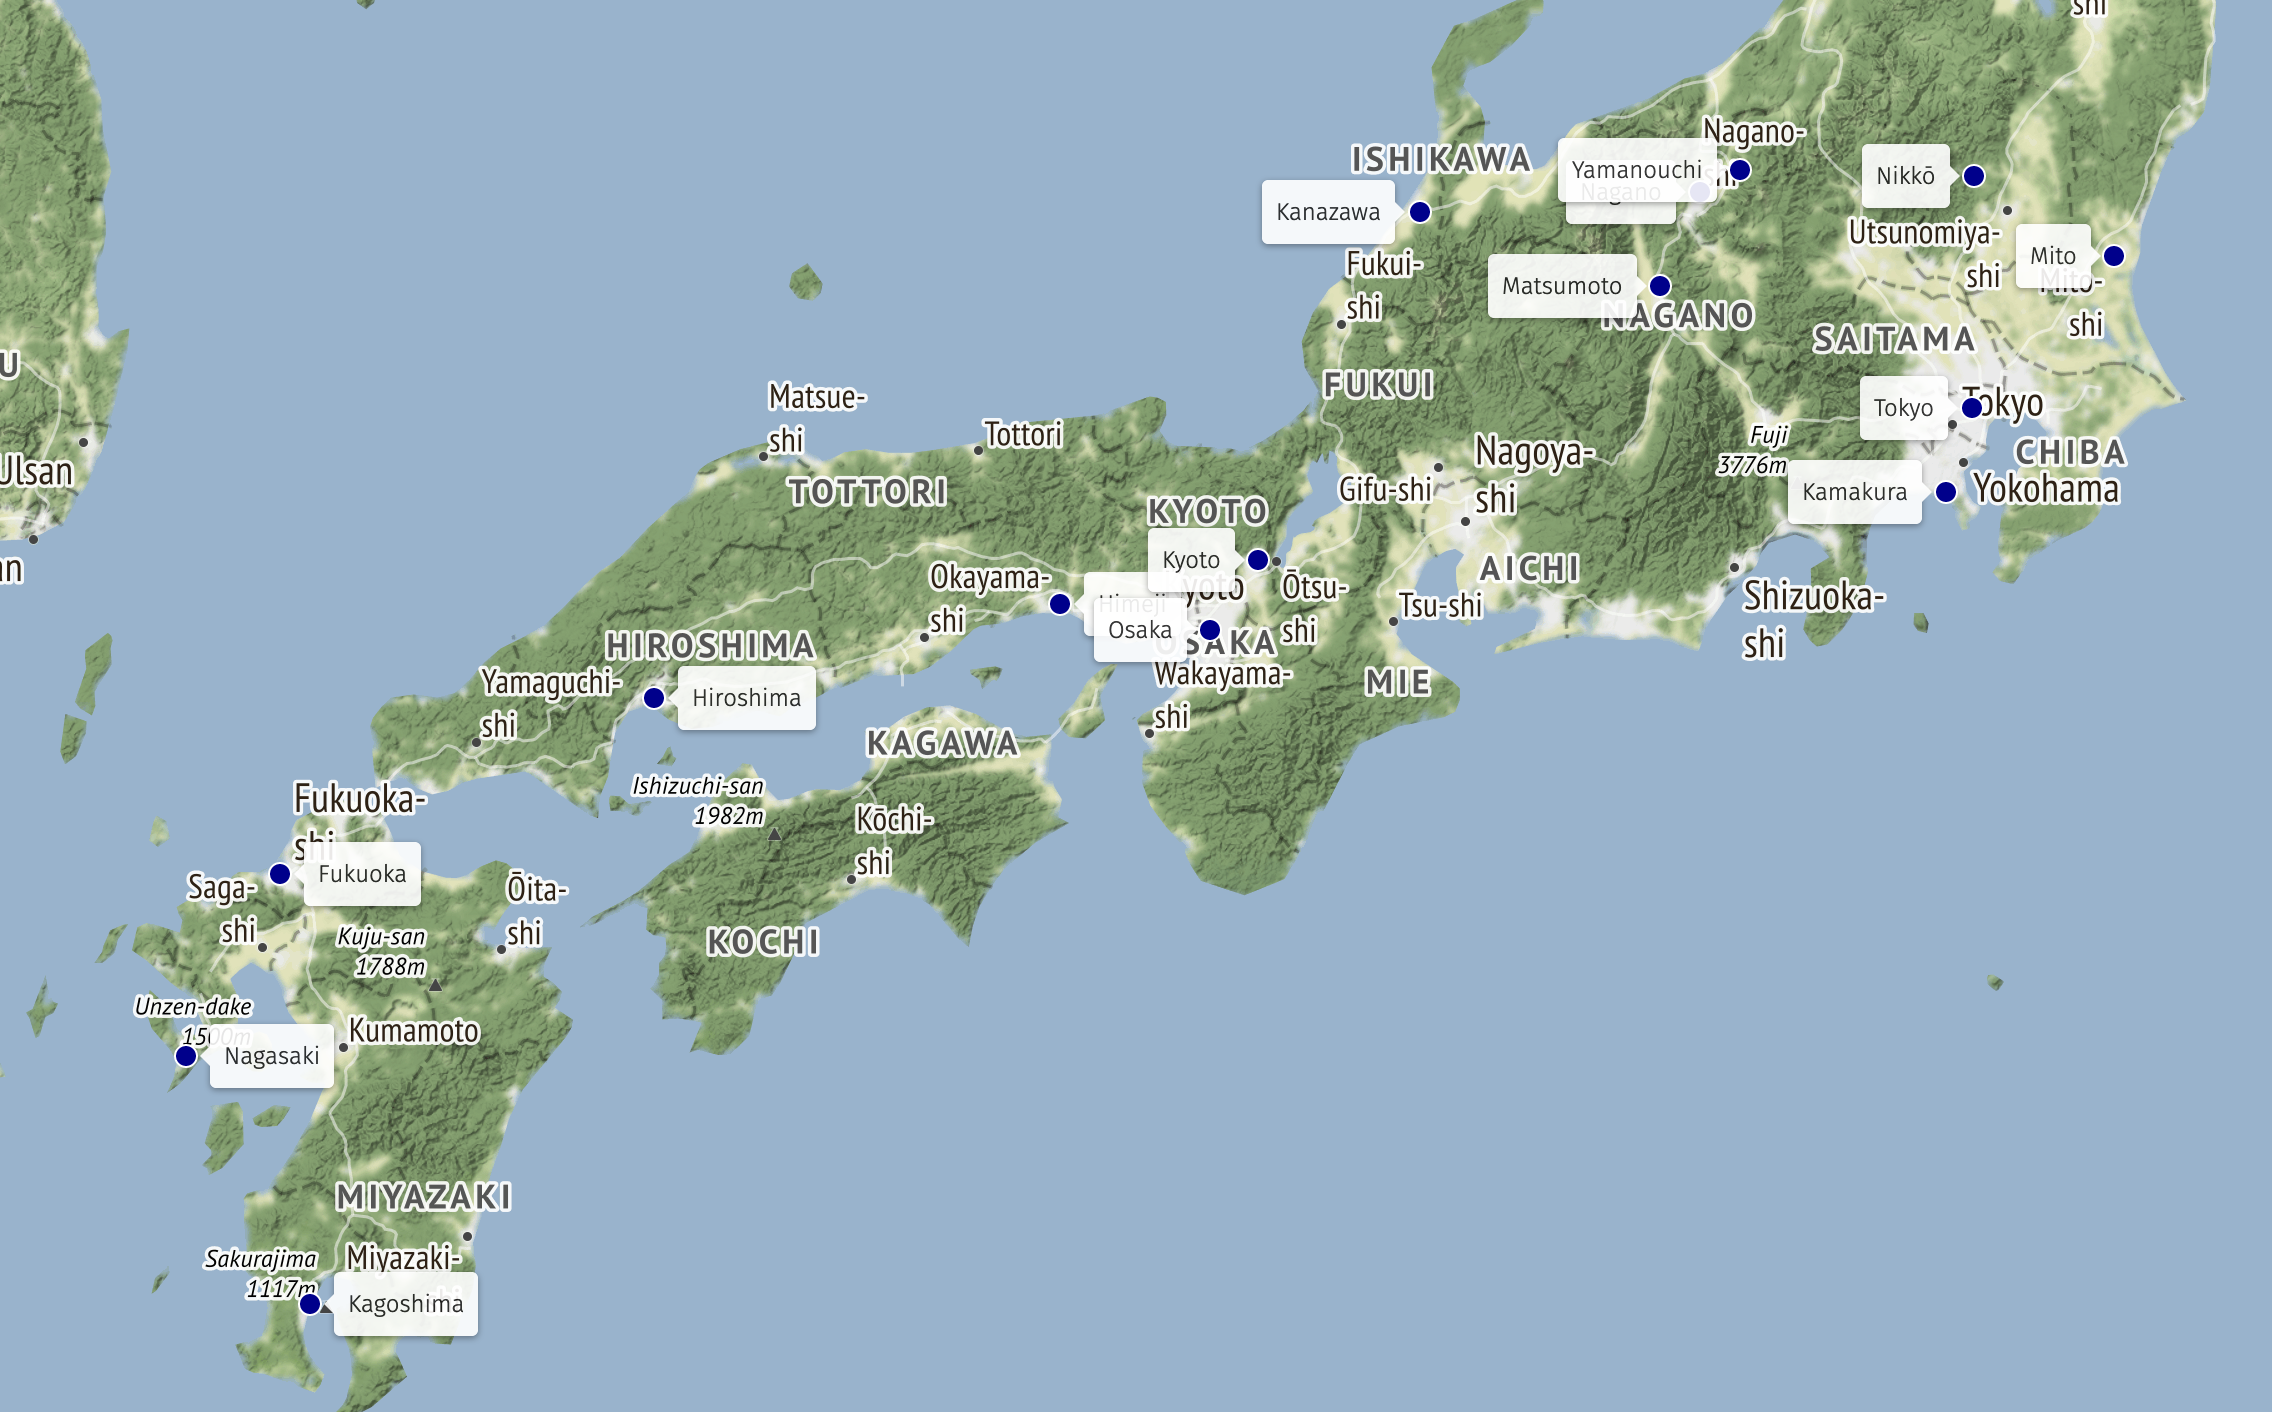
\includegraphics{maps/Japon.png}
\end{figure}

\emph{Elida et Florian}
